\section{Numerical Solution of Equations}

\subsection{The OpenFOAM Code}

The numerical solution of the equations presented in Chapter \ref{chap: equations} was obtained using the OpenFOAM code. Details of OpenFOAM formulation are explained in \cite{jasak} and \cite{weller}.  From all the set of available solvers and libraries in OpenFOAM, the dieselFOAM solver and dieselSpray class were the major pieces of code used in this work. To my knowledge, both were written by Niklas Nordin, \cite{nordin}.

The dieselSpray class handles the modeling of lagrangian particles and their submodels. Minor modifications were made in order to have more flexibility in boundary conditions and to adapt them to the experimental conditions.

The dieselFOAM solver couples the modeling of the lagrangian particles and the gas flow solution. The spray sources are explicitly treated and the coupling among variables is solved with PISO algorithm, see \cite{jasak} and \cite{ferziger}.

Minor modifications were added to the solution of low Mach number equations instead of the fully compressible formulation.
They are briefly explained here, but the understanding requires from the reader some familiarity with OpenFOAM programming.

The thermodynamic pressure retained its original name \verb|p| and is the pressure used in the state equation:
\begin{verbatim}
<createFields.H>
volScalarField& p = thermo.p();                               
\end{verbatim} 
and in the lagrangian models:
\begin{verbatim}
<createSpray.H>
spray dieselSpray
(
    U,
    rho,
    p,
    T,
    composition,
    gasProperties,
    thermo,
    g
);\end{verbatim} 

A new scalar field was assigned to the dynamic pressure, \verb|volumeScalarField pd|:
\begin{verbatim}
<createFields.H>
 volScalarField pd
(
    IOobject
    (
        "pd",
        runTime.timeName(),
        mesh,
        IOobject::MUST_READ,
        IOobject::AUTO_WRITE
    ),
    mesh
);
\end{verbatim} 

The momentum equation was modified to be computed using the gradient of \verb|pd| instead of \verb|p| in the momentum predictor:
\begin{verbatim}
<UEqn.H>
     fvVectorMatrix UEqn
    (
        fvm::ddt(rho, U)
      + fvm::div(phi, U)
      + turbulence->divDevRhoReff(U)
     ==
        rho*g
      + dieselSpray.momentumSource()
    );

    if (momentumPredictor)
    {
        solve(UEqn == -fvc::grad(pd));
    }
\end{verbatim} 

Finally, the the pressure equation is now a Poisson equation for the dynamic pressure and it uses the thermodynamic presure for computing the density.
\begin{verbatim}
<pEqn.H>

  fvScalarMatrix pdEqn
  (
      fvc::ddt(psi,p)
      + fvc::div(phi)
      - fvm::laplacian(rho*rUA, pd)
      ==
      Sevap
  );
\end{verbatim} 
where \verb|psi| or $\Psi$ is the isothermal compressibility. For an ideal gas:
\begin{equation}
 \rho=p\Psi=\frac{p}{RWT} \, .
\end{equation}

In this work, the time-dependence of the thermodynamic pressure is neglected and the therm \verb|fvc::ddt(psi,p)| vanishes.

\section{Aspects of the Numerical Solution}
The calculations deviate from experiments due to three groups of errors as stated in \cite{jasak} and briefly explained here:
 
\begin{description}
 \item[Modeling Errors:] the difference of the real flow and the exact solution of the mathematical model.
 \item[Discretization Errors:] the difference between the exact solution of the mathematical model and the exact solution of the discretized equations on the discretized domain (the numerical grid).
 \item[Iteration Convergence Errors:] the difference between the approximate and the exact solution of the discretized equations in the discretized domain. The approximate solution is obtained by iterative methods that reduce the convergence error up to a certain level known as the solver tolerance. 
 \end{description}
 
 The modeling errors were already discussed as the governing equations were presented in Chapter \ref{chap: equations}. The discretization of equations is treated in next section. The criterion for iteration convergence was set to $10^{-7}$ for the pressure equation and $10^{-6}$ for the remaining variables. The residual of equations were monitored during execution to ensure the validity of the solution.
 
The equations were solved in segregated linear systems using conjugate gradient algorithms. The solution did not present convergence difficulties as the convergence tolerances were satisfied in few iterations.

\subsection{Discretization of the Governing Equations}
The general transport equation for a scalar intensive property $\phi$ is:
\begin{equation}
 \underbrace{\frac{\partial \rho \phi}{\partial t}}_{\text{temporal derivative}} + \underbrace{\nabla \cdot \left(\rho \bv{U} \phi \right)}_{\text{advection}} - \underbrace{\nabla \cdot \left( \rho \Gamma \nabla \phi \right)}_{\text{diffusion}} = \underbrace{S\left(\phi\right)}_{\text{source}}
\end{equation}


Each term was discretized using the following schemes:
\begin{itemize}
 \item Temporal derivative: Euler implicit method;
 \item Advection term: Gauss theorem is applied to transform the divergence in surface integrals and the upwind scheme is used to interpolate cell centered values to cell faces;
 \item Diffusion term: Gauss theorem with linear interpolation from cell center to faces. Central difference is used for the gradient;
 \item Sources: all sprays sources are explicitly handled. The spray is evolved from time step "n" to "n+1" using the gas phase properties at time step "n", and all source terms are computed. The gas is then evolved to time step "n+1".
\end{itemize}

\subsection{Domain Discretization (The Numerical Grid)}

Two axisymmetric (2D) orthogonal mesh grids were built: a fine and a coarse grid. OpenFOAM uses the collocated grid arrangement. The fine grid was composed of $14,800$ cells ($74$ cells in the radial direction and $200$ in the axial direction) and the coarse grid was composed of $5,460$ cells ($42$ in the radial direction and $130$ in the axial direction). The geometries are shown in Figure \ref{fig: meshes}.

\begin{figure}[!htb]
 \centering
 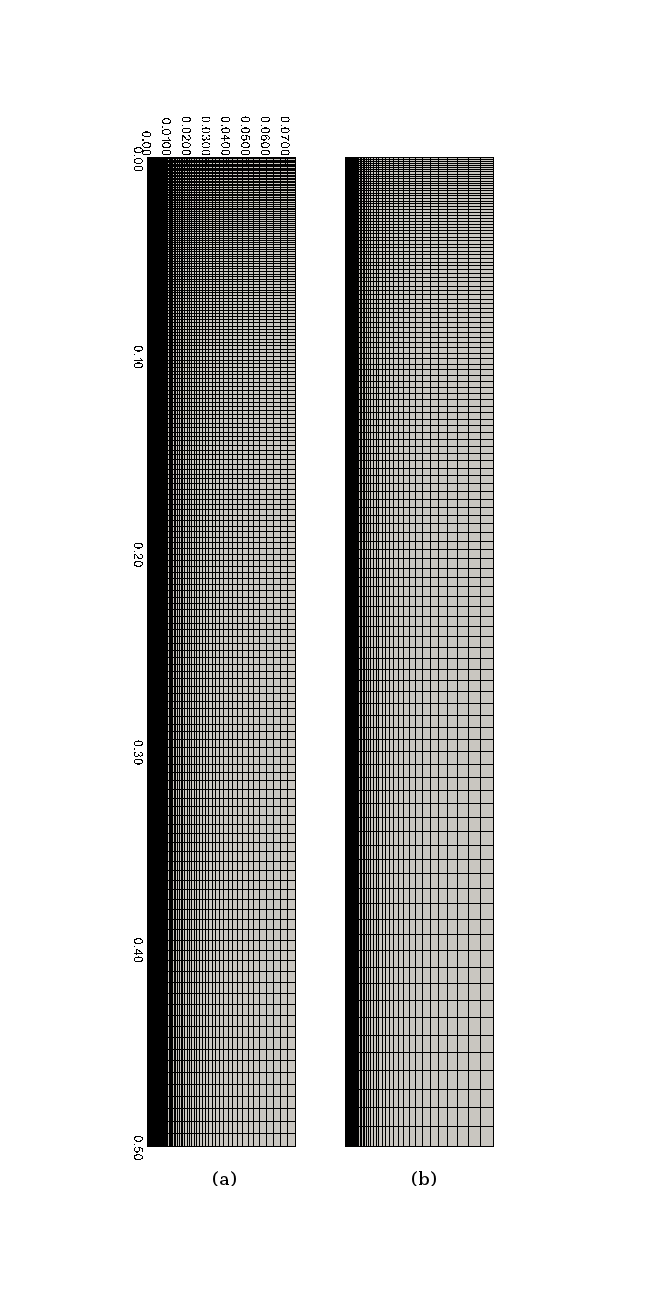
\includegraphics[height=0.9\textheight]{./figuras/chap4/grid.png}
 \caption{Planar view of the fine (a) and the coarse grid (b).}
\label{fig: meshes}
\end{figure}

Solutions for both grids were obtained for a gas phase only flow using the same boundary conditions described in Chapter \ref{chap: exp}, hence the same Reynolds number, and the same discretization schemes for the equations and the same convergence tolerances previously mentioned. 

Figure \ref{fig: grid_test} shows on the left the comparison of radial profiles of mean axial velocity ($\tilde{U}_x$) for the axial coordinates: $x/D=5$, $x/D=15$ and $x/D=25$. In the same Figure, but on the right, it is shown radial profiles of the turbulent kinetic energy ($k$) for the same axial coordinates. In despite of some differences, the coarse grid solution was considered enough accurate and it was used for the results presented in Chapter \ref{chap: results}.

\begin{figure}[h]
 \centering
\begin{tabular}{cc}
 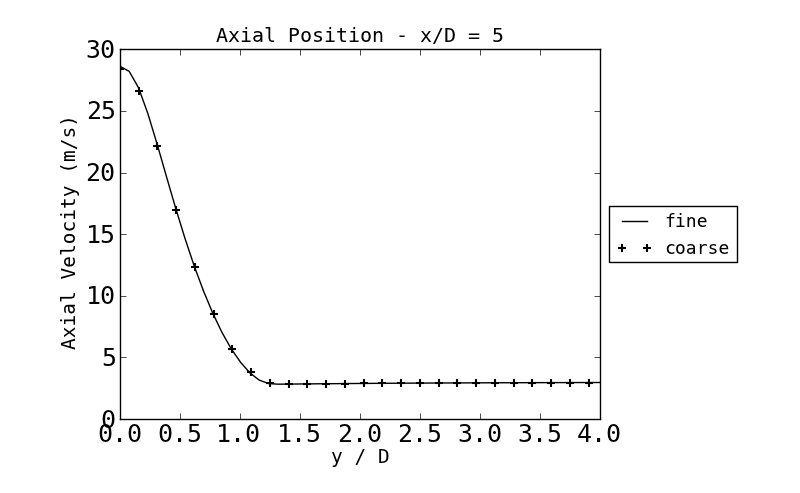
\includegraphics[width=0.5\textwidth]{./figuras/chap4/coarse_fine/grid_0_U.png} & 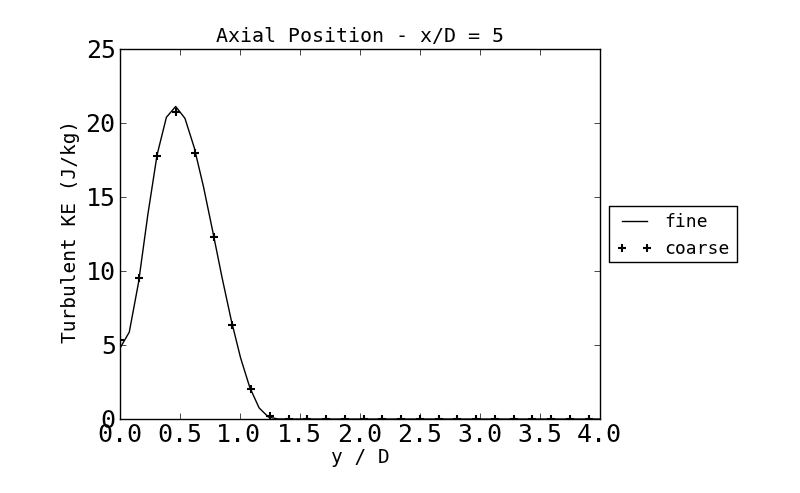
\includegraphics[width=0.5\textwidth]{./figuras/chap4/coarse_fine/grid_0_k.png} \\
(a) & (b) \\
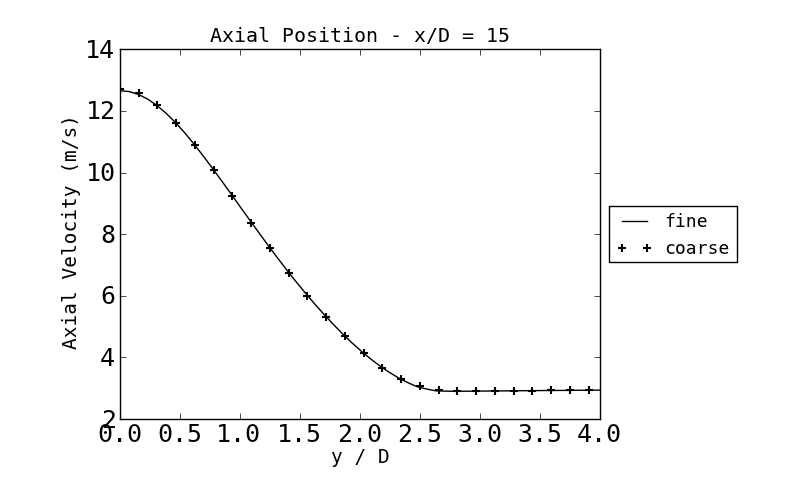
\includegraphics[width=0.5\textwidth]{./figuras/chap4/coarse_fine/grid_2_U.png} & 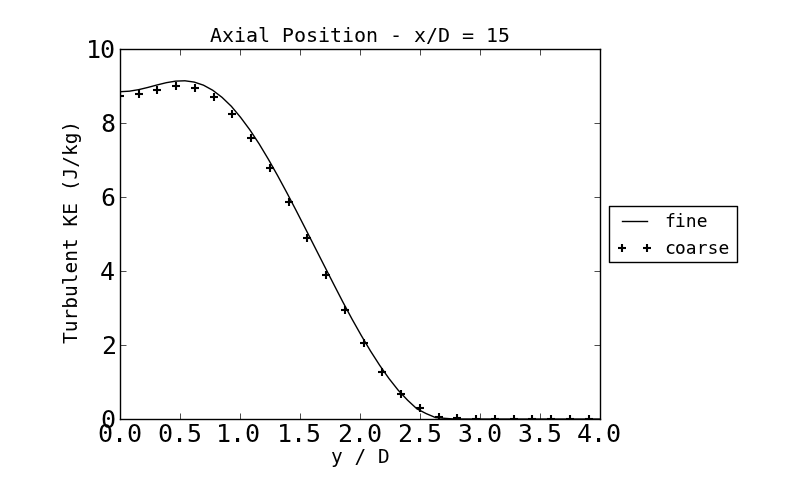
\includegraphics[width=0.5\textwidth]{./figuras/chap4/coarse_fine/grid_2_k.png} \\
(c) & (d) \\
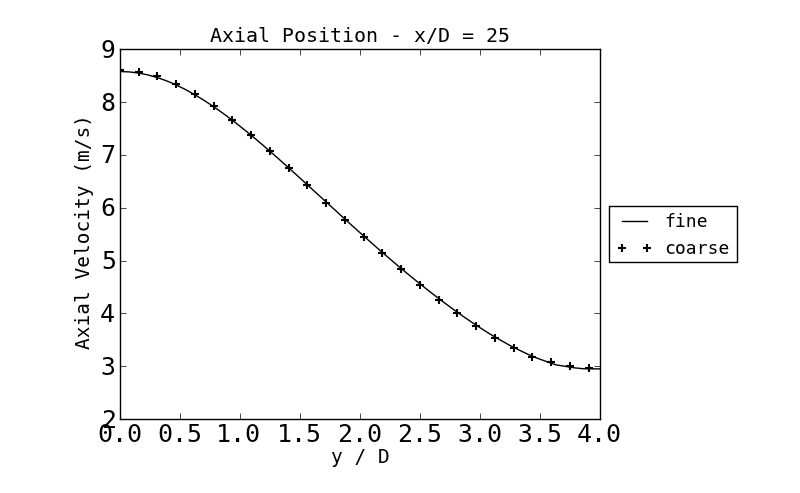
\includegraphics[width=0.5\textwidth]{./figuras/chap4/coarse_fine/grid_4_U.png} &   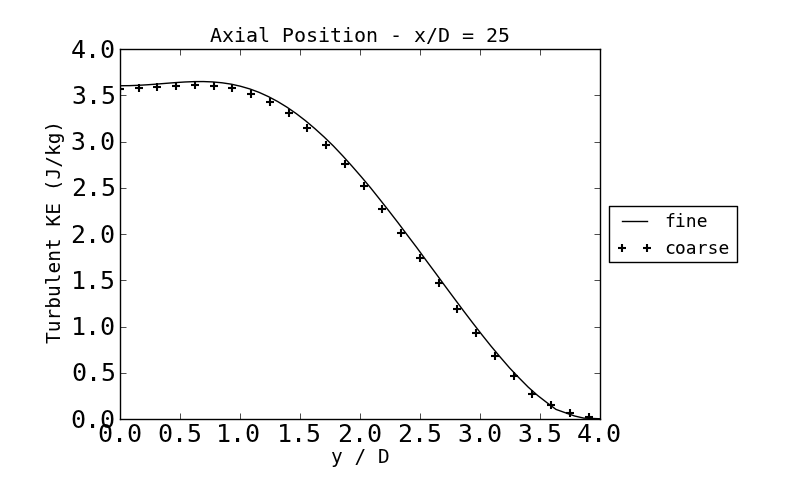
\includegraphics[width=0.5\textwidth]{./figuras/chap4/coarse_fine/grid_4_k.png} \\
(e) & (f)
\end{tabular}
 \caption{Comparison of radial profiles obtained for the fine and the coarse meshes for a pure gaseous jet. Mean axial velocity ($\tilde{U}_x$) on the left for axial coordinates: $x/D=5$ in (a), $x/D=15$ in (c) and $x/D=25$ in (e); and turbulent kinetic energy ($k$) on the right: $x/D=5$ in (b), $x/D=15$ in (d) and $x/D=25$ in (f).}
 \label{fig: grid_test}
\end{figure}

It is not clear how mesh refinements will necessarily improve computations for the lagrangian description of droplets. This happens because it is made the assumption that the liquid volume fraction in the computational cell is negligible. If the mesh is refined further and further, this might become untrue. For the present work, the liquid volumetric fraction in the cells near the nozzle is about $10^{-3}$ for the fine mesh and about $10^{-5}$ for the coarse mesh.

Another problem with mesh refinement using the lagrangian-eulerian approach is the differences obtained in interpolating gas properties to parcel positions from one grid to another. This problem has been discussed in \cite{nordin} and \cite{baumgarten2006mixture}. 

So far, the recommendation for the mesh dependency is to refine the cells until certain accuracy for the continuous phase is satisfied and not until the eventual limitation of computational cost, what could violate the assumption of a low liquid volume fraction.

% DROPLET TRACKING
% PISO ALGORITHM
